\section{Umsetzungskonzept}
Die Grundidee für die Umsetzung der Zebrastreifen Erkennung lässt sich in folgenden Punkten zusammenfassen:
\begin{enumerate}
	\item Download der Strassen- und Zebrastreifenkoordinaten
	\item Download von Orthofotos auf OpenStreetMap Zoomlevel 19
	\item Anfertigen von einheitlichen Bildern entlang der Strassen
	\item Zebrastreifenerkennung mithilfe des Convnets
	\item Vergleich bestehende Zebrastreifen mit neu gefundenen
	\item Parallelisierung des Erkennungsprozesses
	\item Daten in eine Maproulette Challenge umwandeln
\end{enumerate}

\subsection{Open Street Map Anbindung}
Um Daten von Open Street Map zu erhalten, kann man eine Open Street Map Web API ansprechen. Mapquest\footnote{\url{http://open.mapquestapi.com/xapi/}} stellt eine solche Open Street Map API zur Verfügung. Mit dieser Schnittstelle lassen sich via HTTP GET Abfragen starten. Eine Bounding Box und die entsprechenden Open Street Map Tags dienen als Input. Man erhält danach alle Daten in einem einfach zu interpretierenden XML Format. Mit der gleichen Abfrage lassen sich sogar Zebrastreifen und Strassen gleichzeitig herunterladen.

\begin{figure}[H]
	\centering
	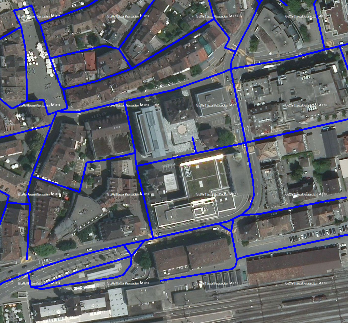
\includegraphics{images/Strassen_Rapperswil.png}
	\caption{Eingezeichnete Strassen in Rapperswil}
\end{figure}

\newpage
\subsection{Bing Anbindung}
Um an die Orthofotos zu kommen, gab es zu Beginn des Projektes mehrere Lösungen:
\begin{enumerate}
	\item Offizielle Microsoft Bing REST Service
	\item Direkter Download über Bing Maps
	\item Benutzung der Orthofotos von der HSR
\end{enumerate}

Als aller erstes haben wir versucht, die Orthosfotos über den offizielle Microsoft Bing REST Service\footnote{\url{https://msdn.microsoft.com/en-us/library/ff701713.aspx}} zu download. Jedoch beschränkt Microsoft den API Zugriff auf 50'000 Transaktionen pro Tag und 125'000 Transaktionen pro Jahr, was uns bei geschätzten 7 Millionen Tiles in der Schweiz nicht reichen würde.

Nachdem diesem ersten Versuch sind wir auf den direkten Download der Othosfotos umgestiegen. Wenn man mit dem Internet Browser auf Bing Maps zugreift, werden die Tiles mithilfe von Javascript von den Bing Servern geladen. Microsoft benutzt das Quadtree\footnote{\url{https://msdn.microsoft.com/en-us/library/bb259689.aspx}} Format, um die entsprechenden Tiles anzusprechen. Mithilfe des Projekts Tiles à la Google Maps\footnote{\url{http://www.maptiler.org/google-maps-coordinates-tile-bounds-projection/}} und der dort zur Verfügung gestellten Python Library, können wir Bounding Boxen in Quadtrees umwandeln.

Die Orthofotos, welche im Besitz der HSR sind und die nur Schweiz umfassen, wären die letzte Lösung gewesen, wenn die anderen Möglichkeiten versagt hätten.

\subsection{Convolutional Neural Network}
Die Evaluation des Suchalgorithmus hat einen klaren Sieger ergeben. Das Convolutional\footnote{Convolutional ist Englisch und heisst auf Deutsch Faltung} Neural Network (hier weiter als Convnet bezeichnet) liefert mit Abstand die besten Resultate innerhalb unserer Test Bounding Box in Rapperswil.

\subsubsection{Geschichte}
Bis noch vor einigen Jahren wurden neuronale Netze zur Bilderkennung grösstenteils ignoriert\footnote{\url{http://karpathy.github.io/2015/10/25/selfie/}}. Das Convnet selbst wurde schon 1980 von einem Japaner namens Fukushima erfunden, jedoch erhielt es keine grössere Beachtung. Hauptgrund dafür war der Rechenhunger für das Training des Netzes. Gedreht hat sich das Ganze erst als 2012 genügend Rechenleistung mithilfe von Grafikkarten zur Verfügung stand. Ab diesem Zeitpunkt erzielte diese wieder gefundene Technik Bestleistungen in vielen Bereichen der Bilderkennung. Bis heute ist das Convnet die präziseste Technik zur Erkennung von Gegenständen in Fotos.

\subsubsection{Funktionsweise}
Ein künstliches neuronales Netz besteht aus einer grossen Anzahl von simulierten Neuronen. Mit verschiedenen Techniken aus der Statistik und  Mathematik kann so ein Input auf einen Output gemappt werden. In unserem Fall wollen wir ein Bild auf eine der Kategorien Crosswalk oder Non-Crosswalk mappen. Dies wird in der Fachliteratur auch Klassifikation von Bildern genannt.

Wie der Name schon sagt, besteht das Convolutional Neuronale Netz aus vielen verschiedenen Faltungsfilter. Ein Faltungsfilter transformiert ein Bild so, dass ein spezifisches Muster auf dem Bild markiert wird. Ein gutes Beispiel für einen Filter ist die Technik der Kantendetektion\footnote{\url{https://de.wikipedia.org/wiki/Kantendetektion}}. Die Kantendetektion markiert nur die Kanten auf dem Bild und ignoriert den restlichen Inhalt.\\

\begin{figure}[H]
	\centering
	
\includegraphics{images/kantendetektion.jpg}
	\caption{Beispiel einer Kantendetektion}
\end{figure}
Ein Convolutional Neuronales Netz lernt nun selbst, welchen Faltungsfilter er anwendet, um das Problem möglichst gut zu lösen. Die extrahierten Muster dienen als Features und werden nun von einem einfachen Neuronalen Netz klassifiziert. Die Ausgabe besteht nun aus aus zwei Werten zwischen 0 und 1. Sie stellen die Wahrscheinlichkeiten der entsprechenden Klasse dar.

\subsubsection{Keras}
Das Projekt Keras\footnote{\url{https://github.com/fchollet/keras}} stellt eine einfache Library zum Entwerfen und Trainieren von Neuronalen Netzen zur Verfügung. Es bietet modulare Funktionen für Convolutional Neuronale Netzwerke und Rekurrente Netzwerke an. Mithilfe eines Flags kann das Training einfach auf die Grafikkarte ausgelagert werden, was bei solchen Algorithmen unerlässlich ist.
\newpage
\subsection{Parallelisierung}
\subsection{Maproulette Challenge}
